\documentclass[twocolumn,amsfont,amssymb,amsmath, showpacs,balancelastpage, nofootinbib]{revtex4-1}
\pdfoutput=1

\usepackage{graphicx}
\usepackage{dcolumn}
\usepackage{bm}
\usepackage{amssymb,amsmath,bm}  
\usepackage{color}
\usepackage[colorlinks,linkcolor=red,citecolor=blue,urlcolor=blue ]{hyperref}
\usepackage{multirow}
\usepackage[utf8]{inputenc}
\usepackage{balance}
\usepackage{enumitem}
\usepackage{lipsum}
\newcommand{\nv}{\hat{\bf n}}

\begin{document}
\title{Science-driven 3D data compression for photometric redshift surveys}
\author{David Alonso$^1$}
\affiliation{$^{1}$Oxford Astrophysics, Department of Physics, Keble Road, Oxford, OX1 3RH, UK}

\begin{abstract}
 \lipsum[0]
\end{abstract}

\maketitle

\section{Introduction}\label{sec:intro}
\lipsum[1]

\section{Method}\label{sec:method}
  A common method to draw cosmological constraints from photometric redshift surveys is to divide the galaxy sample into tomographic redshift bins and use the information encoded in all the relevant auto- and cross-correlations between different bins, making use of various calibration methods in order to estimate the true redshift disitribution of each bin. Several criteria can be followed in order to select these redshift bins, such as minimising the correlation between non-neighbouring bins or preserving a roughly constant number density on all bins. Here we present a formalism to determine an optimal scale-dependent binning scheme based on maximizing the amount of cosmological information.

  \subsection{Tomographic galaxy clustering}\label{ssec:method.tomographic}
    Let us start by assuming that we have split the galaxy sample into $N_s$ subsamples. As mentioned above, we will think of each of these subamples as some kind of redshift binning (e.g. binning galaxies in terms of their maximum-likelihood redshift), but the formalism applies to any set of subsamples. Let $f^\alpha(\nv)$ be the a field on the sphere at the angular position $\nv$ and defined in terms of the properties of the sources in the $\alpha$-th sample (e.g. the cosmic shear field $\gamma^\alpha$ or the galaxy overdensity $\delta^\alpha$), and let $\phi^\alpha(z)$ be the redshift distribution of sources in the sample. Finally, let $a^\alpha_{\ell m}$ be the spherical harmonic coefficients of $f^\alpha$\footnote{Spin-2 fields, such as the cosmic shear, will be decomposed in spin-2 spherical harmonics, however the discussion below holds for this case too}. The power spectrum for our set of subsamples is defined as the two-point correlator of $a^\alpha$:
    \begin{equation}
      \left\langle {\bf a}_{\ell m}\,{\bf a}^\dag_{\ell' m'} \right\rangle\equiv\delta_{\ell\ell'}\delta_{mm'}{\sf C}_\ell,
    \end{equation}
    where we have packaged $a^\alpha$ as a vector for each $(\ell,m)$: ${\bf a}_{\ell m}\equiv(a^1_{\ell m},...,a^{N_s}_{\ell m})$. In general, the observed field will receive contributions from the true cosmological signal (${\bf s}$) and measurement noise (${\bf n}$). Assuming both components are uncorrelated, the same split applies in the power spectrum:
    \begin{equation}
      {\sf C}={\sf S}+{\sf N},\hspace{12pt}
      {\sf S}\equiv\left\langle{\bf s}\,{\bf s}^\dag\right\rangle, \hspace{12pt}
      {\sf N}\equiv\left\langle{\bf n}\,{\bf n}^\dag\right\rangle.
    \end{equation}
  
    Once the choice of subsamples $\alpha$ is chosen, the standard analysis method would then proceed by performing a likelihood evaluation of the two-point statistics of these subsamples. While this procedure is relatively simple, it suffers from a number of drawbacks:
    \begin{enumerate}
      \item It is not clear what the optimal strategy should be to define the sub-samples. One could make sure to exploit all of the information present in the data by using a large number of very narrow redshift bins, and let the likelihood evaluation pick up the information encoded in them. This is however impractical for several reasons.
      \item $C^{\alpha\beta}_\ell$ is a $N_s\times N_s\times N_\ell$ data vector. Thus increasing $N_s$ will increase the computational time required for each likelihood evaluation like $N_s^2$ and number of elements of the covariance matrix of $C^{\alpha\beta}_\ell$ like $N_s^4$, with the corresponding increase in complexity needed to estimate this covariance. Although this can be partially alleviated by considering only correlations between neighbouring redshift shells, the amount of information lost by ditching all correlations beyond a given neighbouring index is not clear in a general setting.
      \item Estimating the redshift distribution for a large number of subsamples can be inaccurate, depending on the method used to do so, on the quality of the photometric redshift posterior information and on the statistics of the spectroscopic sample.
    \end{enumerate}
  
  \subsection{The Karhunen-Loeve basis}\label{ssec:method.klbasis}
    The idea of the method considered here is to form a small number of linear combinations of the data distributed in narrow redshift bins designed to contain the maximum amount of cosmological information. This can be expressed as a generic Karhunen-Loeve eigenvalue problem (e.g. see \cite{1997ApJ...480...22T} for details), and the procedure to determine the coefficients of these linear combinations is relatively simple:
    \begin{enumerate}
      \item We start by assuming that the field ${\bf a}$ has been measured in a number of narrow redshift bins, and by defining the inverse-variance weighted field $\tilde{\bf a}_{\ell m}\equiv{\sf N}^{-1}_\ell\,{\bf a}_{\ell m}$.
      \item Let us consider a (possibly $\ell$-dependent) set of linear combinations of the weighted field measured on narrow redshift bins:
      \begin{equation}
        {\bf b}_{\ell m}={\sf E}_\ell\cdot\tilde{\bf a}_{\ell m}\equiv{\sf E}_\ell\circ{\bf a},
      \end{equation}
      where ${\bf E}_\ell$ is a yet-unspecified matrix and we have defined the non-standart dot product: ${\bf v}^\dag_\ell\circ{\bf w}_\ell\equiv{\bf v}^\dag_\ell\cdot{\sf N}^{-1}_\ell\cdot{\bf w}_\ell$. The power spectrum for this new observable would then simply be given by:
      \begin{equation}
        {\sf D}_\ell\equiv\left\langle{\bf b}_{\ell m}\,{\bf b}^\dag_{\ell m}\right\rangle={\sf E}_\ell^\dag\circ{\bf C}_\ell\circ{\sf E}_\ell.
      \end{equation}
      \item Let us now find the set of orthonormal vectors ${\bf v}^p_\ell)$ (with ${\bf v}^{p\dag}\circ{\bf v}^q=\delta^{pq}$) that diagonalize the cross-shell power spectrum ${\sf C}_\ell$\footnote{Note that this can always be found also in the case of non-standard dot products. Let ${\sf P}$ be the matrix defining the product, and ${\sf P}={\sf L}{\sf L}^T$ its Cholesky decomposition. The problem of diagonalizing a symmetric matrix ${\sf A}$ with respect to this product is equivalent to diagonalizing ${\sf A}'\equiv{\sf L}^T{\sf A}{\sf L}$ with the standard dot product and multiplying the resulting eigenvectors by $\left({\sf L}^T\right)^{-1}$.}. We then identify $({\sf E}_\ell)^p_\alpha$ with the elements of ${\bf v}^p(\ell)$. Note that, after this transformation and without any further optimization, some of the practicalities of the original problem the original problem are already simplified, since we can now focus on the diagonal elements of the new power spectrum and its covariance.
      \item Let's assume that we are interested in measuring a set of cosmological parameters $\Theta\equiv\{\theta_1,...\}$. The information regarding this set of parameters encoded in a given data vector ${\bf x}$ can be quantified in terms of its Fisher matrix (the Hessian of the log-likelihood with respect to $\Theta$), which assuming $\langle{\bf x}\rangle=0$ reads
      \begin{equation}
        F_{ij}\equiv\left\langle\partial_i\partial_j{\cal L}\right\rangle=\frac{1}{2}{\rm Tr}\left(\partial_i{\sf X}\,{\sf X}^{-1}\partial_j{\sf X}\,{\sf X}^{-1}\right),
      \end{equation}
      where ${\sf X}\equiv\langle {\bf x}{\bf x}^T\rangle$ is the covariance matrix of the data. Since the power spectrum of ${\sf b}$ defined above is diagonal, this expression gets simplified further, and the Fisher matrix can be decomposed into the independent contributions of each mode: $F_ij=\sum_p F^p_{ij}$, where
      \begin{align}        
        F^p_{ij}&\equiv\sum_\ell\frac{2\ell+1}{2}\,(\partial_i\log D^p_\ell)\,(\partial_j\log D^p_\ell)
      \end{align}
      Thus we can rank the eigenvectors $({\sf E}_\ell)^p_\alpha$ in terms of their information content (in a Fisher-matrix sense).
      \item We then truncate the number of modes to analyze to the first $M$ eigenmodes thus defined, which should therefore contain the bulk of the information needed to constrain $\Theta$.
    \end{enumerate}
    This strategy therefore allows one to reliably and significantly reduce the dimensionality of the data vector from $N_s^2\times N_\ell$ to $M\times N_\ell$ while minimising the loss of information. Note that, although the method is based on an initial thin-slicing of the galaxy distribution, the fact that the final datased comprises only a small set of samples means that the method is not penalized in terms of photometric redshift uncertainties. The same methods used to calibrate these uncertainties in the standard analysis hold in this case with slight modifications (e.g. weighed and $\ell$-dependent stacking of photo-$z$ pdfs, or cross-correlations of the weighed maps with a spectroscopic survey in the case of clustering redshifts).
  
    \subsubsection{Special case: the harmonic-bessel basis}\label{sssec:method.klbasis.bessel}
      Let us consider a simplified case where $f$ is the overdensity field of a non-evolving galaxy population for which, furthermore, and for which we neglect the effect of redshift-space distortions. Let us further assume that we have perfect redshift information, such that we can split the sample into thin radial slices of equal width $\delta \chi$, which we label by their comoving radius $\chi$. The noise in the measurement of $f$ is given purely by shot noise, and since (as per our initial assumptions) the number density of sources does not change with $r$, the noise power spectrum is diagonal and scales like 
      \begin{equation}
        N_\ell(r,r')\propto \frac{\delta_{r,r'}}{r^2}.
      \end{equation}
      Thus, the dot product is just given by:
      \begin{equation}
        {\bf b}^\dag\circ{\bf c}\propto\int dr\,r^2\,b(r)^*\,c(r).
      \end{equation}
    
      In this case, the cross-shell power spectrum is given by,
      \begin{equation}
        C_\ell^{rr'}=\frac{2}{\pi}\int_0^\infty dk\,k^2\,P_k\,j_\ell(kr)j_\ell(kr'),
      \end{equation}
      and it is trivial to show that the K-L eigenmodes are simply given by the spherical Bessel functions: $({\sf E}_\ell)^k_r\propto \sqrt{2/\pi}j_\ell(kr)$:
      \begin{widetext}
      \begin{align}
        D_\ell^{kk'}&\propto\frac{2}{\pi}\int dr\,r^2\int dr'\,r'^2 j_\ell(kr)j_\ell(k'r') C_\ell^{rr'}\\
        &=\int dq\,q^2P_q\left[\frac{2}{\pi}\int dr\,r^2\,j_\ell(qr)j_\ell(kr)\right]\left[\frac{2}{\pi}\int dr'\,r'^2\,j_\ell(qr')j_\ell(k'r')\right]\\
        &=\int dq\,q^2P_q\frac{\delta(k-q)}{q^2}\frac{\delta(k'-q)}{q^2}=P_k\frac{\delta(k-k')}{k^2}=\frac{P_k}{k^2\Delta k}\delta_{k,k'}
      \end{align}
      \end{widetext}
   
      This choice of basis defines the so-called harmonic-Bessel decomposition, and has been postulated as a possible data-compression method for the analysis of photometric redshift data (CITES here). In any realistic scenario (e.g. in the presence of redshift uncertainties, RSDs or for the analysis of weak lensing data), this basis is, however, non-optimal in terms of information loss, as opposed to the K-L basis described above.

\section{Performance}\label{sec:results}
  Here we explore the performance of this method in a number of specific science cases.
  
  \subsection{Weak lensing - K-L basis for dark energy}\label{ssec:results.wl}
    \begin{figure*}
      \centering
      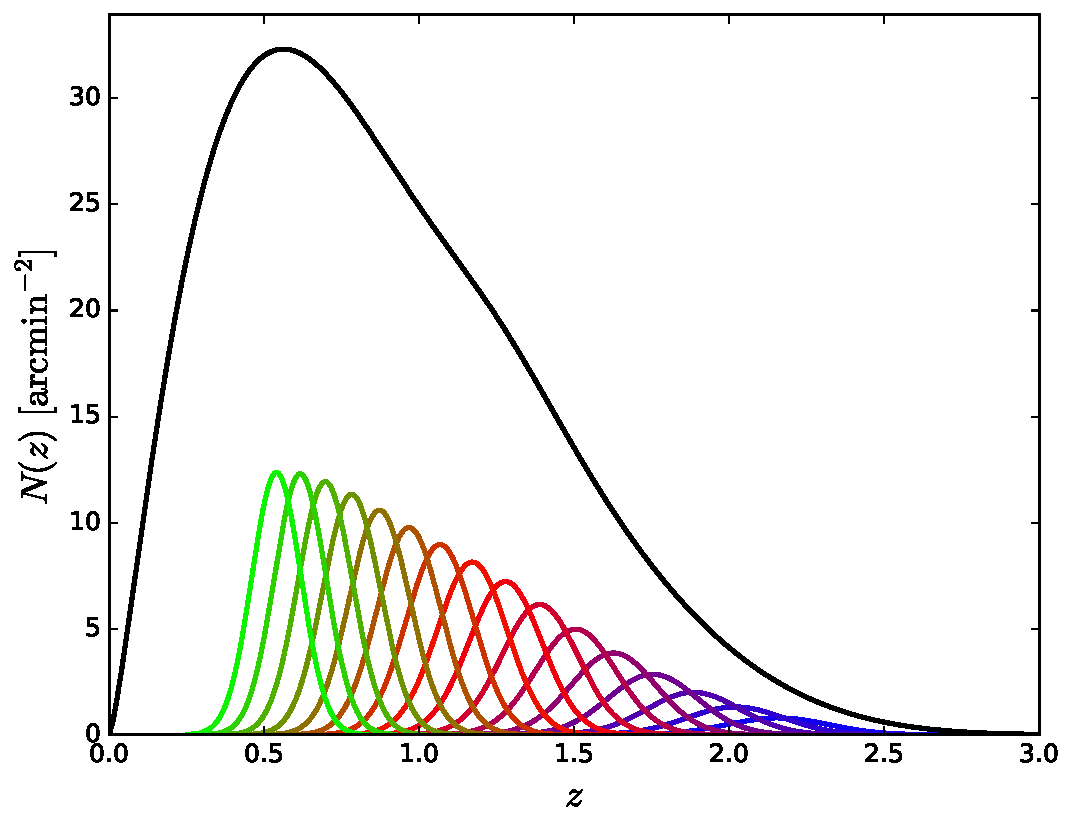
\includegraphics[width=0.49\textwidth]{Figs/nz_lsst_wl}
      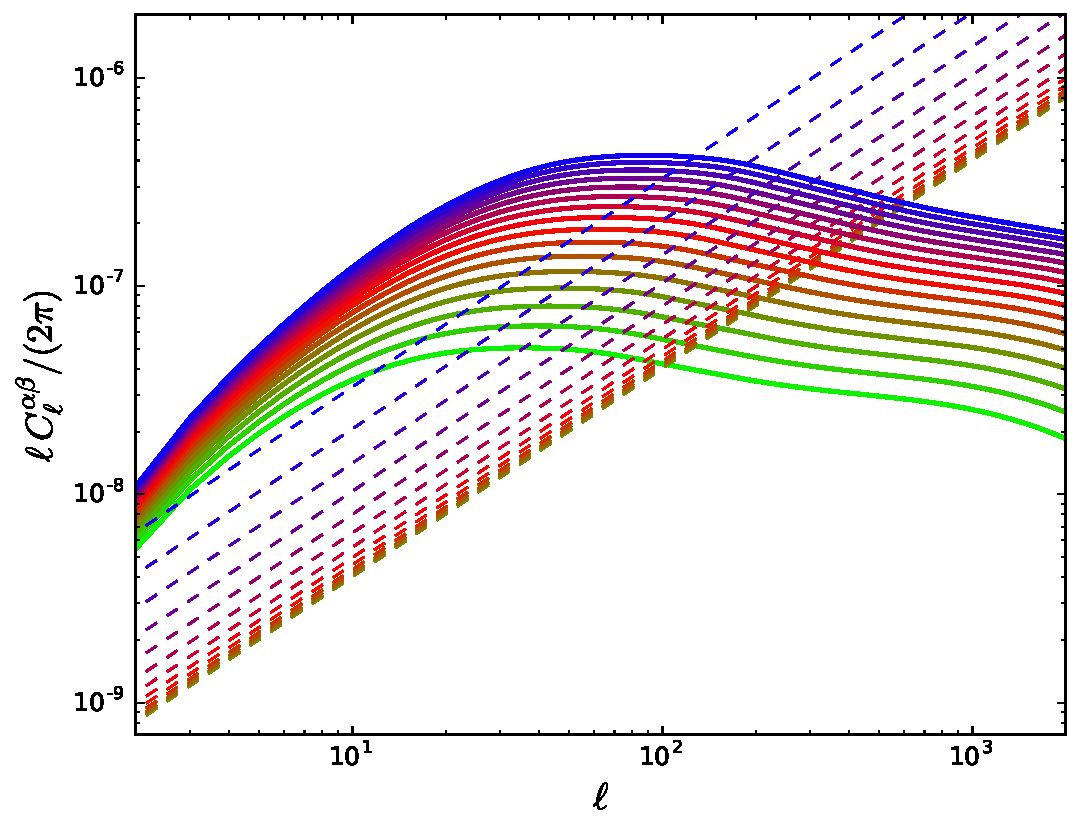
\includegraphics[width=0.49\textwidth]{Figs/c_ij_wl}
      \caption{}\label{fig:nz_wl}
    \end{figure*}
    \begin{figure}
      \centering
      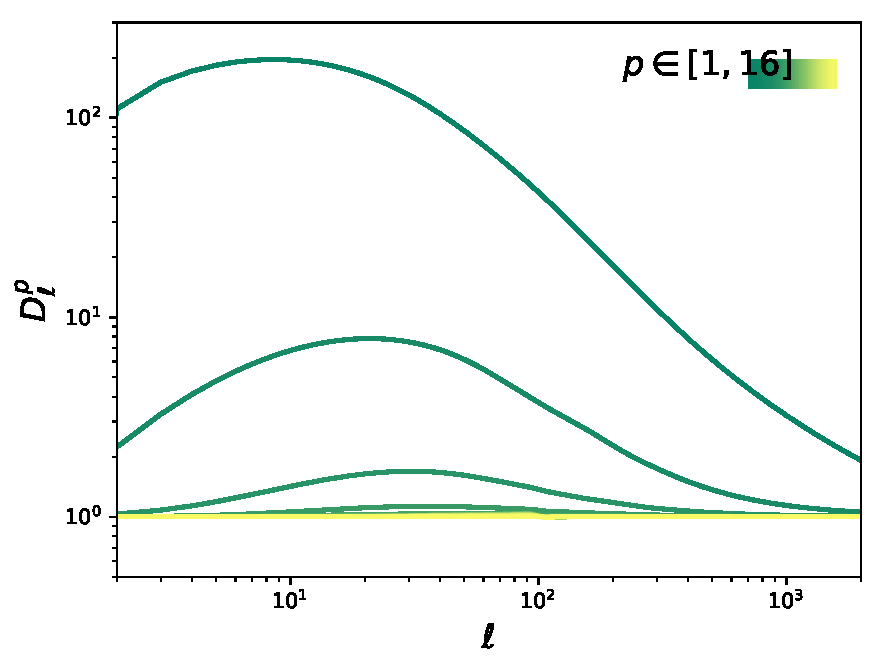
\includegraphics[width=0.49\textwidth]{Figs/d_p_wl}
      \caption{}\label{fig:dp_wl}
    \end{figure}
    \begin{figure*}
      \centering
      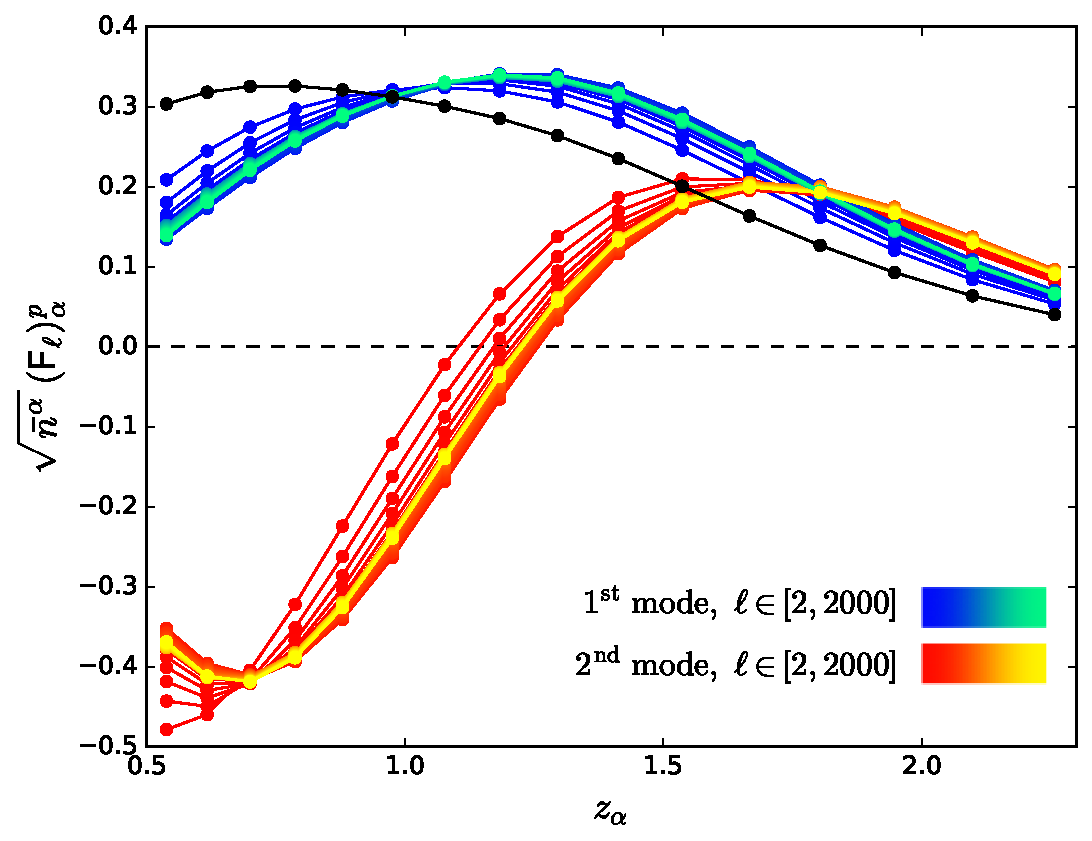
\includegraphics[width=0.49\textwidth]{Figs/kl_modes_wl}
      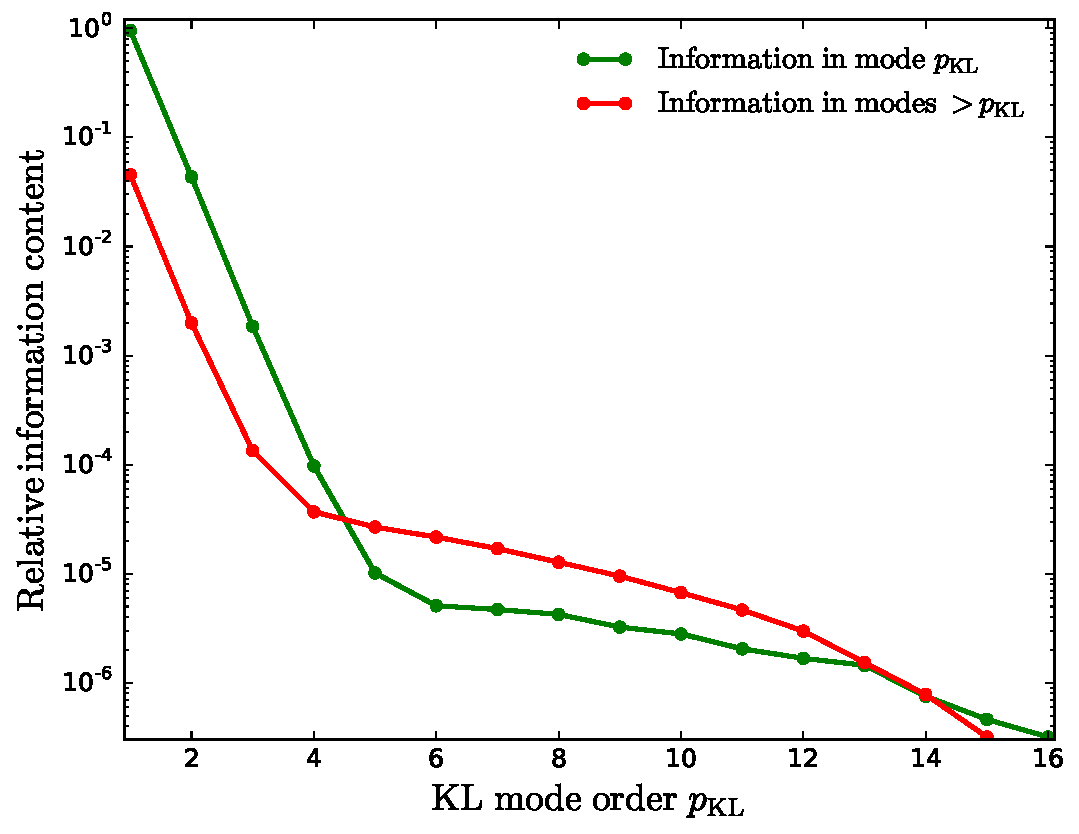
\includegraphics[width=0.49\textwidth]{Figs/information_wl}
      \caption{}\label{fig:kl_wl}
    \end{figure*}
    To quantify the performance of the K-L modes for weak lensing we study the case of an LSST-like survey. The survey specifications and the characteristics of the galaxy sample are described in detail in CITE. In summary, we assume a sample with $\sim29$ objects per ${\rm arcmin}^2$ with the redshift distribution shown in Figure FIG. We also approximate the photo-$z$ distribution as Gaussian with a scatter $\sigma_z=0.05\,(1+z)$.    
    
    The signal part of the cross-power spectrum between the cosmic shear measurements made in two different redshift shells is given by:
    \begin{equation}
      S^{\alpha\beta}_\ell=\frac{2}{\pi}\int_0^\infty dk\,k^2\,\Delta^\alpha_\ell(k)\Delta^\beta_\ell(k),
    \end{equation}
    where the transfer functions $\Delta^{\alpha}_\ell$ take the form:
    \begin{widetext}
    \begin{align}
      \Delta^{\gamma,\alpha}_\ell(k)\equiv\frac{3H_0^2\Omega_M}{2k^2}\sqrt{\frac{(\ell+2)!}{(\ell-2)!}}\int d\chi\,W^\alpha(\chi)\frac{j_\ell(k\chi)}{\chi\,a(\chi)}\sqrt{P(k,z(\chi))},\hspace{12pt}
      W^\alpha(\chi)\equiv\int_{z(\chi)}^\infty dz\,\phi^\alpha(z)\frac{\chi(z')-\chi}{\chi(z')\chi}.
    \end{align}
    \end{widetext}
    Here $\phi^\alpha(z)$ is the redshift distribution of sources in the $\alpha$-th bin. The noise power spectrum is white and simply given by the intrinsic ellipticity scatter weighed by the number density of sources in each redshift bin $\bar{n}^\alpha$:
    \begin{equation}
      N^{\alpha\beta}_\ell=\delta_{\alpha\beta}\frac{\sigma_\gamma^2}{\bar{n}^\alpha},
    \end{equation}
    with $\bar{n}^\alpha$ in units of ${\rm srad}^{-1}$. We use $\sigma_\gamma=0.28$.
    
    As our initial set of narrow redshift bins, we select top-hat bins in photo-$z$ space for $z_{\rm ph}>0.5$ with a width given by the value of $\sigma_z/2$ at the center of the bin. The resulting set of 33 bins is shown in Figure FIG. The large overlap between bins implies that a thinner slices is unlikely to unveil significantly more information (an assumption that we verify below). The lensing auto-power spectra (both signal and noise) for these bins are shown in the left panel of Figure FIG.
    
    We compute the K-L modes for this setup and rank them according to their information content on the dark energy equation of state $w$. The diagonal power spectra for the resulting set of modes is shown in the right panel of  Figure FIG.  Comparing against the left panel of the same figure we can see that the K-L decomposition effectively separates the signal-dominated and noise-dominated modes. The fractional contribution of each mode to the total constraint on $w$ (i.e. its contribution to the corresponding Fisher matrix element) is shown in the left panel of Figure FIG. Most of the information ($\sim95\%$) is contained within a single mode, and the first two modes are able to recover more than $99\%$ of the total. The eigenvectors corresponding to the first mode for different values of $\ell$ are shown in the right panel of the same Figure. The eigenvector upweights the parts of the redshift range with the highest signal-to-noise penalising the low-$z$ regime due to its poor lensing signal and the high-$z$ bins due to their high shot noise.

  \subsection{Galaxy clustering - measuring $f_{\rm NL}$}\label{ssec:results.fnl}
    \begin{widetext}
    \begin{equation}
      \Delta^{\delta,\alpha}_\ell(k)\equiv\int dz\,\phi^\alpha(z)\left[b^\alpha(z)j_\ell(k\,\chi(z))-f(z)j_\ell''(k\,\chi(z))\right]\,\sqrt{P(k,z)}
    \end{equation}
    \end{widetext}
    Here $b^\alpha(z)$ is the galaxy bias and $f(z)\equiv d\log\delta/d\log a$ is the growth rate of structure (we have kept the contribution from redshift-space distortions at linear order but ignored the effect of magnification bias).

\section{Discussion}\label{sec:discussion}
  \lipsum[2]

\section*{Acknowledgements}
  \lipsum[3]
  
\bibliography{paper}

\appendix
\section{Pseudo-$C_\ell$ estimation of the K-L modes}\label{app:pcl}
  One of the standard methods to estimate the angular power spectrum of any two quantities in the cut sky is the so-called pseudo-$C_\ell$ estimator. This section adapts this method to the modes resulting from the K-L decomposition described before.
  
  The standard pseudo-$C_\ell$ method is based on computing the spherical harmonic coefficients of the mask field:
  \begin{equation}
    \tilde{a}^\alpha_{\ell m}=\int d\nv\,a^\alpha(\nv)\,w^\alpha(\nv),
  \end{equation}
  where $w^\alpha$ is the weights map characterizing the mask of the field $a^\alpha$. One then estimates the power spectrum of this object by averaging over $m$ for each $\ell$:
  \begin{equation}
    \tilde{C}^{\alpha\beta}_\ell\equiv\frac{\sum_m\tilde{a}^\alpha_{\ell m}\tilde{a}^{\beta *}_{\ell m}}{2\ell+1}.
  \end{equation}
  This object is then related to the true underlying power spectrum through a mode-coupling matrix $M^{\alpha\beta}_{\ell\ell'}$ such that
  \begin{equation}
    \tilde{C}^{\alpha\beta}_\ell=\sum_{\ell'}M^{\alpha\beta}_{\ell\ell'}C^{\alpha\beta}_{\ell'},\hspace{12pt}
    M^{\alpha\beta}_{\ell \ell'}\equiv\sum_{\ell''}\frac{(2\ell'+1)(2\ell''+1)}{4\pi}W^{\alpha\beta}_{\ell''}
    \left(
    \begin{array}{ccc}
      \ell & \ell' & \ell''\\
      0 & 0 & 0
    \end{array}
    \right)^2
  \end{equation}
  where the coupling matrix $M$ depends solely on the power spectrum of the masks $W^{\alpha\beta}_\ell\equiv(2\ell+1)^{-1}\sum_mw^\alpha_{\ell m}w^{\beta *}_{\ell m}$.
  
  The extension of this estimator to the power spectrum of the K-L modes is straightforward: we project the masked harmonic coefficients $\tilde{a}^\alpha$ over the K-L eigenvectors ${\sf E}$ (i.e. $\tilde{\bf b}_{\ell m}\equiv {\sf E}_\ell\circ\tilde{\bf a}_{\ell m}$) and compute their power spectra by averaging over $m$. The resulting estimator takes the form $\tilde{D}^p_\ell=\sum_{\ell'}M_{\ell\ell'}^{pp'}D^{p'}_{\ell'}$, where the new mode-coupling matrix is given by:
  \begin{equation}
    M^{pp'}_{\ell\ell'}\equiv M^{\alpha\beta}_{\ell\ell'}\left[({\sf E}_\ell)^p_\alpha({\sf N}^{-1})_{\alpha\alpha'}({\sf E}_{\ell'})^{p'}_{\alpha'}\right]\left[({\sf E}_\ell)^p_\beta({\sf N}^{-1})_{\beta\beta'}({\sf E}_{\ell'})^{p'}_{\beta'}\right]
    =M_{\ell\ell'}\left[({\sf E}_\ell)^p_\alpha({\sf N}^{-1}_\ell)_{\alpha\beta}({\sf E}_{\ell'})^{p'}_\beta\right]^2
  \end{equation}
  where the second equality holds only if all the maps $a^\alpha_\ell$ share the same mask $w$.\footnote{Note that, for full-sky coverage $M_{\ell\ell'}=\delta_{\ell\ell'}$ and using the orthonormality of ${\sf E}$ we get $M^{pp'}_{\ell\ell'}=\delta_{\ell\ell'}\delta_{pp'}$.}

\end{document}
